\section{Результаты измерений}
\subsection{Центровка элементов оптической системы}
\begin{tabular}{|c|c|c|c|c|}
\hline
    Линза & 1 & 2 & 3 & 4 \\\hline
    Приблизительное $F,\;\text{см}$ & $5$ -- $7$ & $15$ & $20$ & рассеивающая \\\hline
    $F,\;\text{см}$ & $7{,}7 \pm 0{,}1$ & $14{,}3 \pm 0{,}1$ & $19{,}5 \pm 0{,}1$ & $-8{,}5 \pm 1{,}4$ \\\hline
\end{tabular}

Для грубого определения фокусного расстояния получали изображение от лампы на поверхности стола и замеряли расстояние от линзы до поверхности. Та, которая не дала изображения~--- рассеивающая.

Для более точного определения фокусных расстояний поместили линзу 1 поместили так, чтобы она создавала параллельный пучок от источника (диафрагму почти полностью закрыли) и создавая точку на экране. Расстояние от линзы до экрана~--- фокусное.

\subsection{Определение фокусных расстояний при помощи экрана}
\begin{figure}[ht!]
    \center{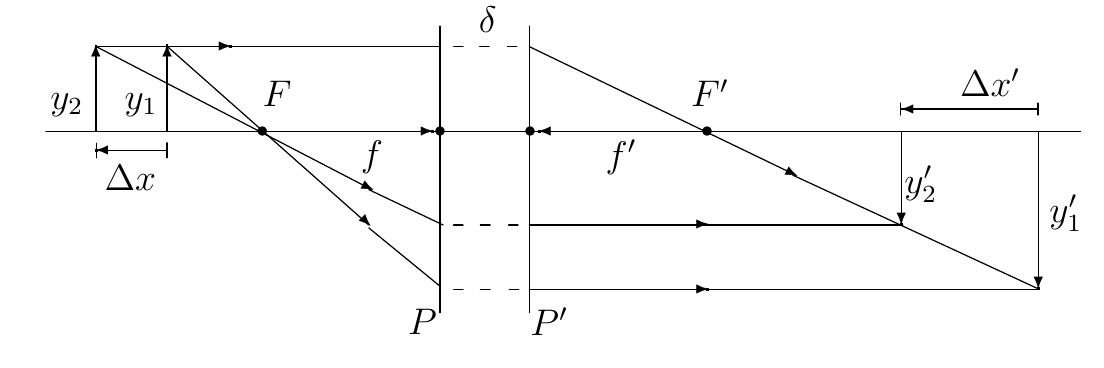
\includegraphics[width=0.8\linewidth]{../img/1.png}}
\end{figure}
Определим фокусное расстояние 1 линзы методом Аббе. $y_{1} = y_{2} = 2{,}0\pm 0{,}05\;\text{см}$.

\begin{tabular}{|c|c|c|}
\hline
     & 1 & 2 \\\hline
    $f,\pm 0{,}5\;\text{см}$ & $17$ & $42{,}5$ \\\hline
    $d,\pm 0{,}5\;\text{см}$  & $12{,}5$ & $9{,}5$ \\\hline
    $y',\pm 0{,}05\;\text{см}$ & $2{,}7$ & $8{,}9$ \\\hline
\end{tabular}

$\Delta x = d_{2} - d_{1} = -3\pm 1\;\text{см}$
$\Delta x' = f_{2} - f_{1} = 25\pm 1\;\text{см}$
$F_{1} = \frac{\Delta x}{y_{1} / y_{1}' - y_{2}/y_{2}'} = 5\pm 2\;\text{см}$
$F_{2} = \frac{\Delta x'}{y_{1}' / y_{1} - y_{2}' / y_{2}} = 8{,}0 \pm 0{,}4\;\text{см}$.

Полученные фокусные расстояния для первой линзы заметно отличаются друг от друга. Это может быть связано с неточностями в измерении расстояний от предмета до линзы и от линзы до изображения.

\begin{figure}[ht!]
    \center{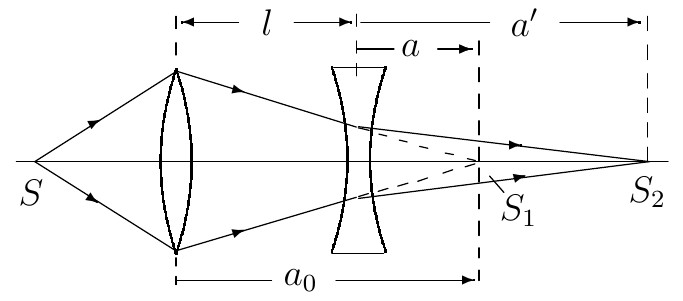
\includegraphics[width=0.8\linewidth]{../img/2.png}}
\end{figure}
Для определения фокусного расстояния рассеивающей линзы соберем схему, изображенную на рисунке.
$a_{0} = 44{,}5 \pm 0{,}5\;\text{см}$, $a' = 19{,}5 \pm 0{,}5 \;\text{см}$, $l = 38{,}5 \pm 0{,}5 \;\text{см}$.
\[
    \frac{1}{F} = -\frac{1}{a_{0} - l} + \frac{1}{a'}
\]
$F = -8{,}5 \pm 1{,}4\;\text{см}$

\subsection{Определение фокусного расстояния и положения главных и фокальных плоскостей сложной оптической системы}

$l_{12} = 5\pm 0{,}1\;\text{см}$, $l_{2} = 3{,}5 \pm 0{,}1\;\text{см}$, $l_{1} = 10{,}3 \pm 0{,}1 \;\text{см}$, $y_{1}' = 5,0 \pm 0{,}1\;\text{см}$, $y_{2}' = 1{,}4 \pm 0{,}1 \;\text{см}$, $x_{1} = 25{,}5 \pm 0{,}1 \;\text{см}$, $x_{2} = 13{,}4 \pm 0{,}1\;\text{см}$.

$\Delta x = -6{,}8 \pm 0{,}2 \;\text{см}$, $\Delta x' = -12{,}1 \pm 0{,}2 \;\text{см}$.

\[
    F_{1} = \frac{\Delta x}{y_{1} / y_{1}' - y_{2} / y_{2}'} =  6{,}6 \pm 0{,}4\;\text{см}
\]
\[
    F_{2} = \frac{\Delta x'}{y_{2}' / y_{2} - y_{1}' / y_{1}} = 6{,}7 \pm 0{,}4\;\text{см} 
\]
\[
    \frac{1}{F_{3}} = \frac{1}{F_{1}} + \frac{1}{F_{2}} - \frac{l_{12}}{F_{1}F_{2}}
\]
\[
    F_{3} = 6{,}5 \pm 0{,}2\;\text{см}
\]

Пункт 14 выполнялся для линз 2 и 3, т.к. линзы 1 и 2 давали слишком большую оптическую силу.
$x_{1} = 6 \pm 0{,}1\;\text{см}$.
В обратную сторону пустить луч не получилось из-за выступающего винта регулировки линзы 3.
